\documentclass[12pt,letterpaper]{article}
\usepackage[margin=1in]{geometry}
\usepackage{fancyhdr}
\usepackage[utf8]{inputenc}
\usepackage{palatino}
\usepackage{microtype}
\usepackage{hyperref}
\usepackage{graphicx}
\usepackage{lastpage}
\usepackage[hang,small]{caption}
\usepackage{titlesec}
\usepackage{amsmath,amssymb}
\usepackage{multirow}
\usepackage{float}

\renewcommand{\headrulewidth}{0pt}
\fancyfoot{}
\fancyfoot[C]{\sf Page \thepage\ of \pageref{LastPage}}
\pagestyle{fancy}

%\titleformat{\section}{\bfseries\Large}{\arabic{\thesection}}{1em}{}
%\titleformat{\subsection}{\bfseries\large}{\arabic{\thesection}.\arabic{\thesubsection}}{1em}{}
%\titleformat{\subsubsection}{\itshape}{\arabic{\thesection}.\arabic{\thesubsection}.\arabic{\thesubsubsection}}{1em}{}

\setlength{\parindent}{0cm}
\setlength{\parskip}{0.8em}

\captionsetup[figure]{labelfont=it,font=it}
\captionsetup[table]{labelfont={it,sc},font={it,sc}}

\hypersetup{colorlinks,
    linkcolor = black,
    citecolor = black,
    urlcolor  = black}
\urlstyle{same}

\title{Performance Analysis of \\ GPU-Accelerated Optical Flow}
\date{December 8, 2014}
\author{Hari Caushik, Kyle Cesare, Soo-Hyun Yoo}



\begin{document}

\maketitle
\thispagestyle{empty}
\newpage

\tableofcontents
\newpage

\section{Abstract}
GPUs, or graphical processing units, have been shown to provide a significant
performance boost over CPUs for highly parallel tasks\cite{gpupipeline}. This
project investigates the performance difference between optical flow algorithms
run on an Intel Core i5 quad core CPU and those run on an NVIDIA Tegra K1 SoC.
We expected the K1 to run these optical flow algorithms significantly faster due
to its ability to parallelize with its GPU. We expect to test the performance
on the Farneback dense optical flow algorithm. This algorithm will process
video frames captured by a GoPro webcam with a USB interface. The performance
metric we will be measuring is frame processing rate.

\section{Graphical Processing Units (GPUs)}
GPUs have been used to improve the performance of a variety of different
applications. While CPUs consist of a few powerful cores optimized for serial
processing, GPUs have a massively parallel architecture consisting of many
smaller, more efficient cores designed for handling multiple tasks
simultaneously\cite{gpuoverview}. We expect the optical flow program to run many
orders of magnitude faster on a GPU than on a CPU, as it can process more arrays
of pixels simultaneously.

\section{Optical Flow}
Optical flow is a problem within the field of Computer Vision concerned with
detecting motion by finding and tracking features or segments across different
images\cite{opticalflowtechniques}. Specifically, this involves measuring the
motion of specific pixel brightness patterns in a sequence of images
\cite{opticalflowtechniques}. Optical flow has many applications
in 3D vision tasks like obstacle avoidance and time-to-collision calculations
\cite{opticalflowgpu}. Performing such calculations at high speed is especially
useful in dynamic systems such as aerial vehicles, which can drift on the order
of meters per second due to sensor noise, external perturbations, or control
inputs.

Optical flow can be sparse or dense. Sparse Optical Flow is the tracking of
a few select pixels in a set of images. Dense Optical Flow is the tracking of
all pixels in a set of images, a much more computationally intensive task.

In this project, we use the Farneback Dense Optical Flow Algorithm, which
computes a polynomial expansion for a neighborhood of pixels and from that
polynomial approximation, computes displacement (or motion) fields using linear
algebra\cite{farneback}. Since the motion fields depend on the size of the
neighborhood, changing this parameter will produce different motion fields and
will probably have an effect on the performance of the flow computation.

We will specifically measure the number of frames processed per second using
both platforms. We use OpenCV and its GPU acceleration compiler option to 
implement this program.

\begin{figure}[H]
  \centering
  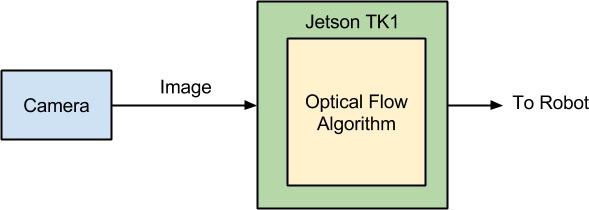
\includegraphics[width=0.8\textwidth]{img/sys.png}
  \caption{Test setup with Jetson devboard processing video stream as input and producing optical flow estimate as output.}
  \label{fig:sys}
\end{figure}

\section{Hardware}
The Nvidia Jetson TK1 development board used in this project is built around
the Nvidia Tegra K1 SoC, which contains a Kepler-based GPU with 192 CUDA cores
and a quad-core ARM Cortex-A15 processor.

\section{Testing Methodology}
To test the criteria outlined above, we will create two programs to produce
identical outputs, but one will target a CPU and the other a GPU. An example of
the program's output is provided in Figure~\ref{fig:flow}.

\begin{figure}[h]
  \centering
  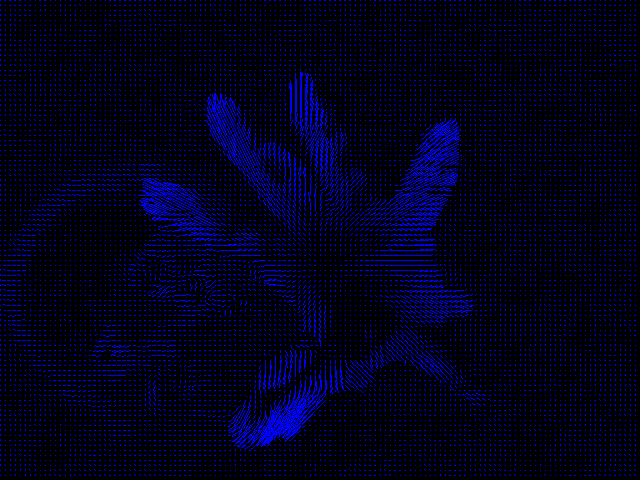
\includegraphics[width=0.8\textwidth]{img/flow.png}
  \caption{An example output image of our testing program.}
  \label{fig:flow}
\end{figure}

To try to identify strengths and weaknesses of each target, we will attempt to
introduce additional variables that may have an impact on performance. These
variables will be:

\begin{description}
  \item[Image resolution] To process a very small image, the overhead required
    to copy memory between the CPU and GPU may be larger than the actual
    processing time. We will use video at QVGA (320x240), VGA (640x480) and FHD
    (1920x1080) to see if this effect is significant.
  \item[Block size] The block size determines the area over which a polynomial
    estimation will be fitted. For a larger block size, fewer polynomials need
    to be computed but each polynomial is more difficult to compute. We want to
    see what this relationship looks like.
\end{description}

It is important to note that the processing times for the first few frames will
be discarded to remove any caching oddities and to allow the GPU kernels to
finish load.

\section{Results}

We first tested the CPU and GPU implementations with constant block size and
various input resolutions (Figures~\ref{fig:cpures}, \ref{fig:gpures}). We then
compared the two implementations given a constant resolution and various block
sizes (Figures~\ref{fig:cpublock}, \ref{fig:gpublock}). Loading times of
individual samples on the GPU at 640x480 resolution with block size of 13 is
shown in Figure~\ref{fig:cudaload}.
% TODO(kyle): Summarize results

\begin{figure}[H]
  \centering
    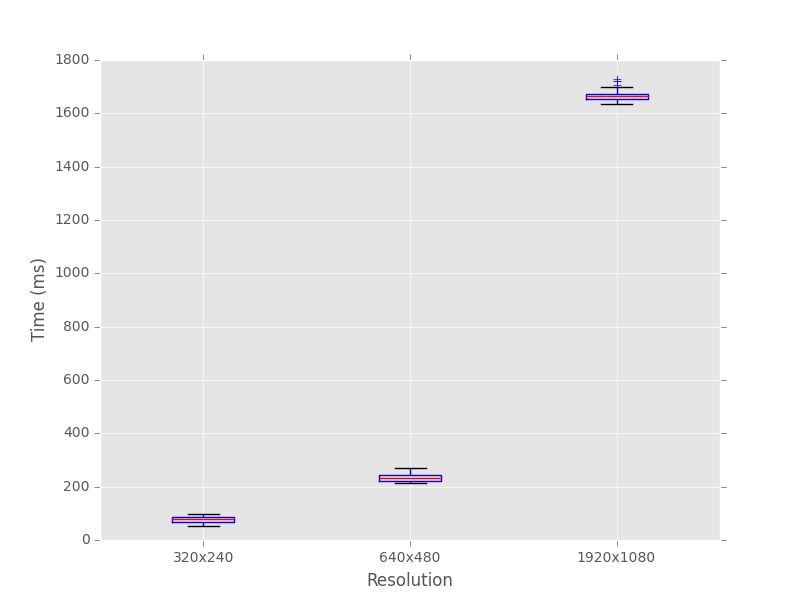
\includegraphics[width=0.8\textwidth]{img/cpu_resolution.png}
  \caption{CPU processing time per frame at block size of 13 and various resolutions.}
  \label{fig:cpures}
\end{figure}

\begin{figure}[H]
  \centering
    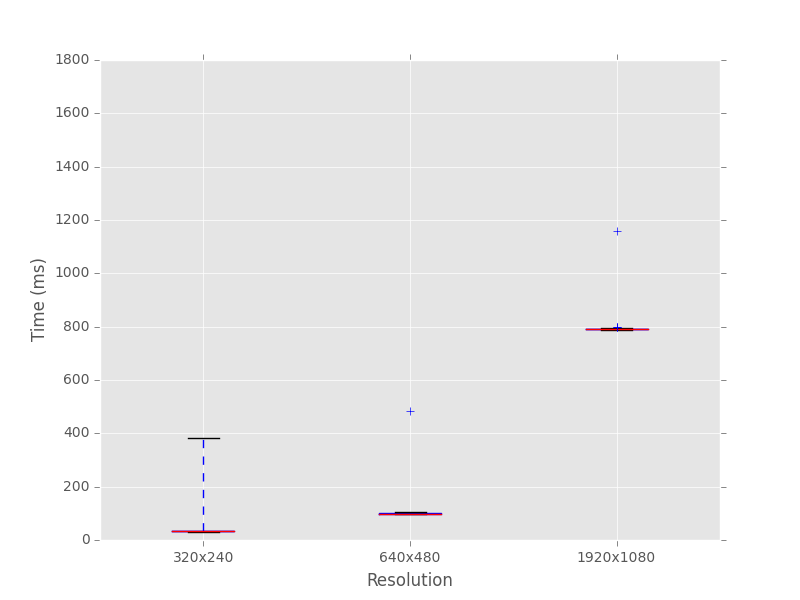
\includegraphics[width=0.8\textwidth]{img/gpu_resolution.png}
  \caption{GPU processing time per frame at block size of 13 and various resolutions.}
  \label{fig:gpures}
\end{figure}

\begin{figure}[H]
  \centering
    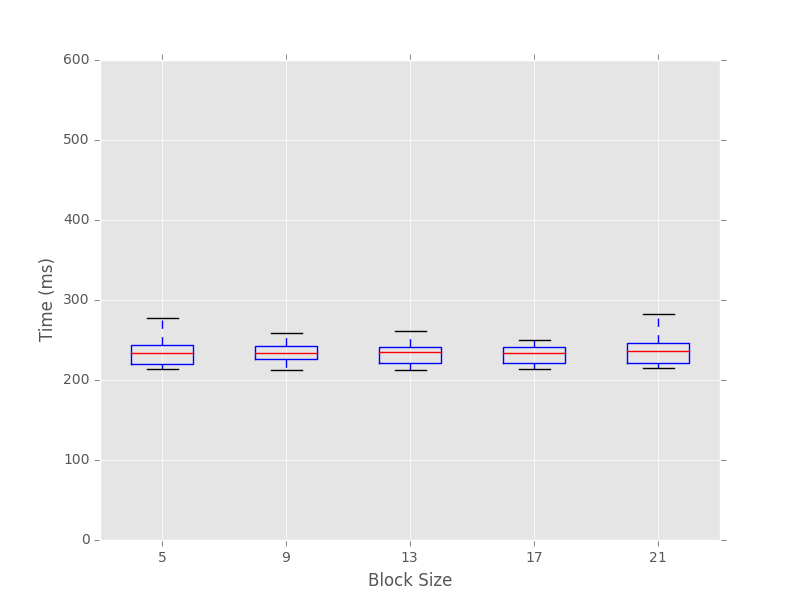
\includegraphics[width=0.8\textwidth]{img/cpu_blocksize.png}
  \caption{CPU processing time per frame at 640x480 resolution and various block sizes.}
  \label{fig:cpublock}
\end{figure}

\begin{figure}[H]
  \centering
    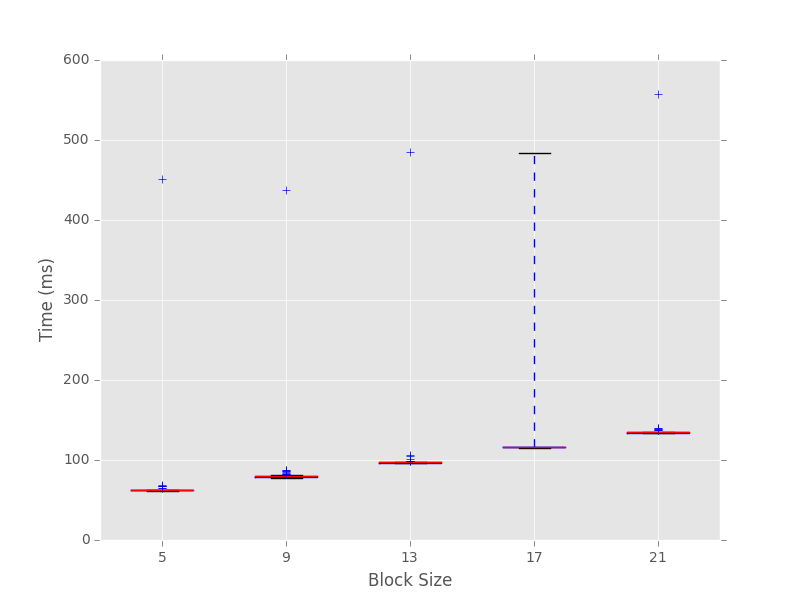
\includegraphics[width=0.8\textwidth]{img/gpu_blocksize.png}
  \caption{GPU processing time per frame at 640x480 resolution and various block sizes.}
  \label{fig:gpublock}
\end{figure}

\begin{figure}[H]
  \centering
    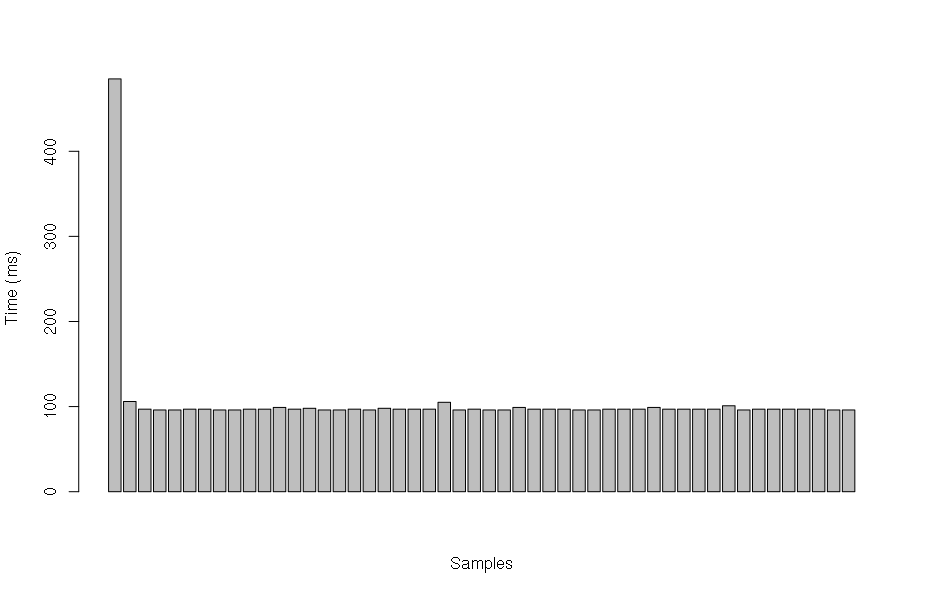
\includegraphics[width=0.8\textwidth]{img/cudaloading.png}
  \caption{GPU processing time for 50 samples at 640x480 resolution and block size of 13.}
  \label{fig:cudaload}
\end{figure}

\section{Implementation Analysis}
To provide more insight into why the GPU showed better performance results than
the CPU, we will now break down the OpenCV Farneback optical flow implementation
used in the trials. We use the \texttt{objdump} tool to disassemble the OpenCV
shared library into an x86 assembly representation. We then use this assembly
code to gather information on the types and counts of instructions being run.

The heavy use of Streaming SIMD Extensions (SSE) makes it more difficult to
reason about the number of floating point operations being performed. An example
of how SIMD executes a single instruction on an array of data is shown in
Figure~\ref{fig:simd}.

\begin{figure}[h]
  \centering
    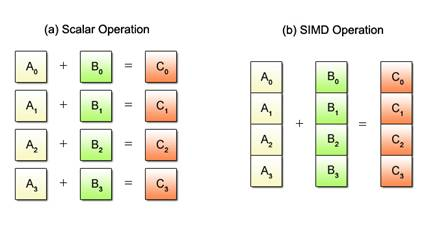
\includegraphics[width=0.8\textwidth]{img/simd.jpg}
  \caption{Illustration of single instruction, multiple data (SIMD)~\cite{simd}.}
  \label{fig:simd}
\end{figure}

The heart of the OpenCV Farneback optical flow implementation is the
\texttt{FarnebackPolyExp} function. While there are other operations that
execute floating point operations, this function is the most expensive. The
number of floating point operations in the core loop is given by:

$$
\text{FP Operations} = \text{levels} * \text{img\_width} * \text{img\_height}
                * (12 + \text{poly\_n} * 17)
$$

For a 1920x1080 image with $\text{levels}=5$ and $\text{poly\_n}=5$, this results in
1,005,696,000 floating point operations per frame. On top of this is several
Gaussian blur operations, several image resizes, and lots of memory access and
allocation.

\section{Conclusion}
Overall, the GPU performed better for all the different image resolutions and
block sizes. The GPU performed about 2x faster for all different resolutions.
It was interesting to note that the CPU processing times for varying block 
sizes remained steady at about 220 ms while the GPU processing times 
increased steadily from about 50 ms to 150 ms when increasing the block size
from about 5 to 21. This could be explained by the fact that a smaller block 
size means more polyfit calculations that can be computed independently
of the other blocks. The GPU is able to take more advantage of parallelism in
this case while for larger block sizes, there are less polyfit calculations to 
compute and thus less computation that can be executed in parallel. In the case
of the CPU, the size of the block and the number of polyfit computations 
seemed to even out and did not show a significant difference across multiple 
block sizes. 

Another interesting result is the variance of the processing times at each 
block size. The CPU processing times varied by about 20 ms across iterations at
each block size while for the GPU, the variance was about 10 ms. This can be
explained by the context switches executed by the Operating System (OS) running
on the CPU. 

The GPU computations contain outliers in figures 4 and 6. Note that the loading
times are constant at about 400 ms for each resolution in figure 4. This is due
to the GPU kernel loading time, the time it takes to copy the kernels, or the
functions to be run on the GPU, to GPU memory. For each frame that the GPU 
optical flow algorithm must process, it must 
\begin{enumerate}
    \item Load the kernels from CPU memory to GPU memory
    \item Transfer the images from CPU to GPU
    \item Perform the optical flow
\end{enumerate}
Since the optical flow kernel is same for each optical flow calculation, the
loading time is constant. The load only needs to be performed for the first 
first frame processed. The GPU only performs steps 2 and 3 for subsequent 
frames.

Not surprisingly, the GPU outperformed the CPU for optical flow computations at
varying image resolutions and block sizes. To extend the work presented in this
paper, it would be interesting to investigate a larger range of block sizes and
image resolutions as well as more CPU and GPU platforms. It may also be useful
to compare performance differences for different optical flow algorithms. 
\section{References}
\nocite{*}
\bibliographystyle{plain-annote}
\bibliography{paper}
%\begin{thebibliography}{10}
%  \bibitem{gpuoverview}
%    http://www.nvidia.com/object/what-is-gpu-computing.html
%  \bibitem{gpupipeline}
%    http://www.cs.virginia.edu/~gfx/papers/paper.php?paper\_id=59
%  \bibitem{jetson}
%    http://www.nvidia.com/object/jetson-tk1-embedded-dev-kit.html
%  \bibitem{opticalflowgpu}
%    Real-Time Optical Flow Calculations on FPGA and GPU Architectures: A Comparison
%    Study
%  \bibitem{opticalflowtechniques}
%   wwww.dgp.toronto.edu/~donovan/stabilization/opticalflow.pdf
%  \bibitem{farneback}
%    Two-Frame Motion Estimation Based on Polynomial Expansion
%  \bibitem{simd}
%    https://www.kernel.org/pub/linux/kernel/people/geoff/cell/ps3-linux-docs/CellProgrammingTutorial/BasicsOfSIMDProgramming.html
%\end{thebibliography}
\end{document}
